%!TEX root = ../Master.tex

\section{Localization}

Localization is used when a given robot has no idea of where it is located. The localization tasks consists of two main tasks; sensing and moving. These two tasks are performed alternately as illustrated in \ref{fig:main tasks}. The robot might have an initial belief of where it is located and in that case this belief is taken into account together with the sense task at first.

\begin{figure}[h]
\centering
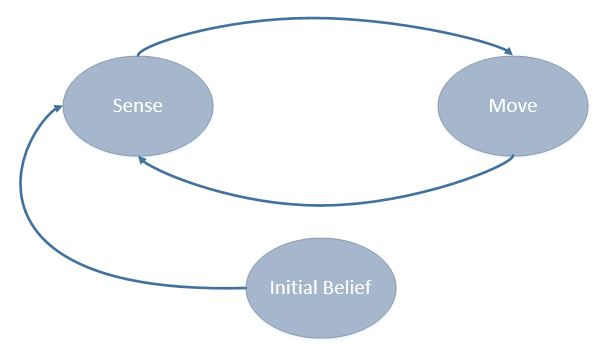
\includegraphics[scale=0.45]{images/SenseMoveInitialBelief}
\caption{Main tasks of localization}
\label{fig:main tasks}
\end{figure}

For the robot to use localization it must be in possession of a map of the environment. The robot uses the map to compare it's belief of it's localization with the map and the results of the sensing.\\

The first task for the robot is to sense. This in done by using the sensors which are built in to the robot. For an example the robot could meassure the distance to all walls in the environment or the color of the floor. These meassurements should lead to a better belief of where the robot is located. Every time the robot senses it gains information of where it is located. The second task for the robot is to move. The robot needs to move in order to be able to get new information from the sensing task. When the robot moves it looses information of where it is located. This is due to inaccuracy of the robots speed and orientation. This will be illustrated in a robot example later on in this section.\\

The algorithm to implement the two tasks is called the Markov Localization algorithm and is illustrated in \ref{fig:markovLocalization}. The algorithm calculates the new belief based on the old belief $bel(x_{(t-1)})$, the motion $u_t$, the meassurements $z_t$ and the map.

\begin{figure}[h]
\centering
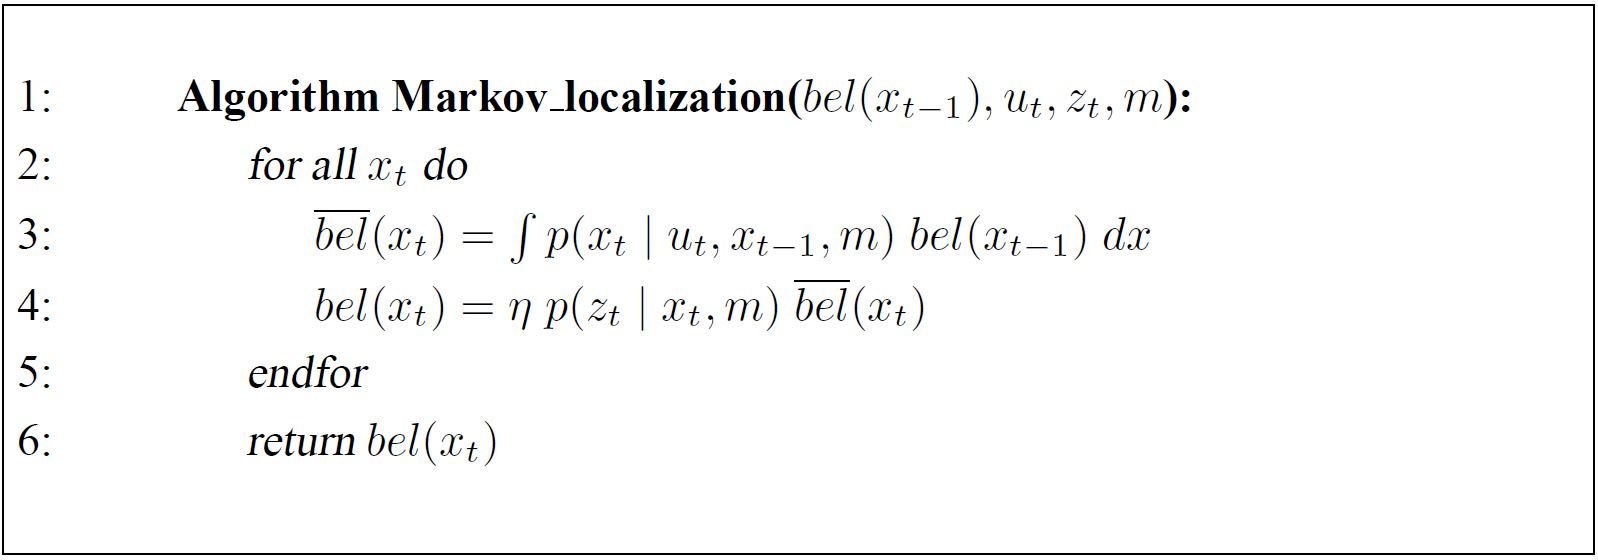
\includegraphics[scale=0.25]{images/MarkovLocalization}
\caption{The Markov Localization algorithm}
\label{fig:markovLocalization}
\end{figure}

The algorithm takes the probability of being located at the new location $x_t$ based on the movement, the prior localization and the map. (Side 175 i bogen)

\subsection{Robot Example}

\begin{figure}[h]
\centering
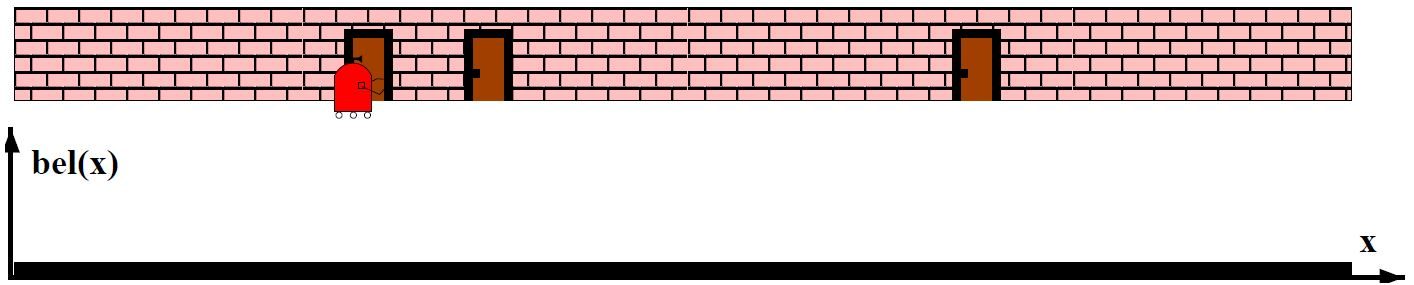
\includegraphics[scale=0.37]{images/MarkovLocalizationA}
\caption{The robot's initial belief}
\label{fig:initialBelief}
\end{figure}

\begin{figure}[h]
\centering
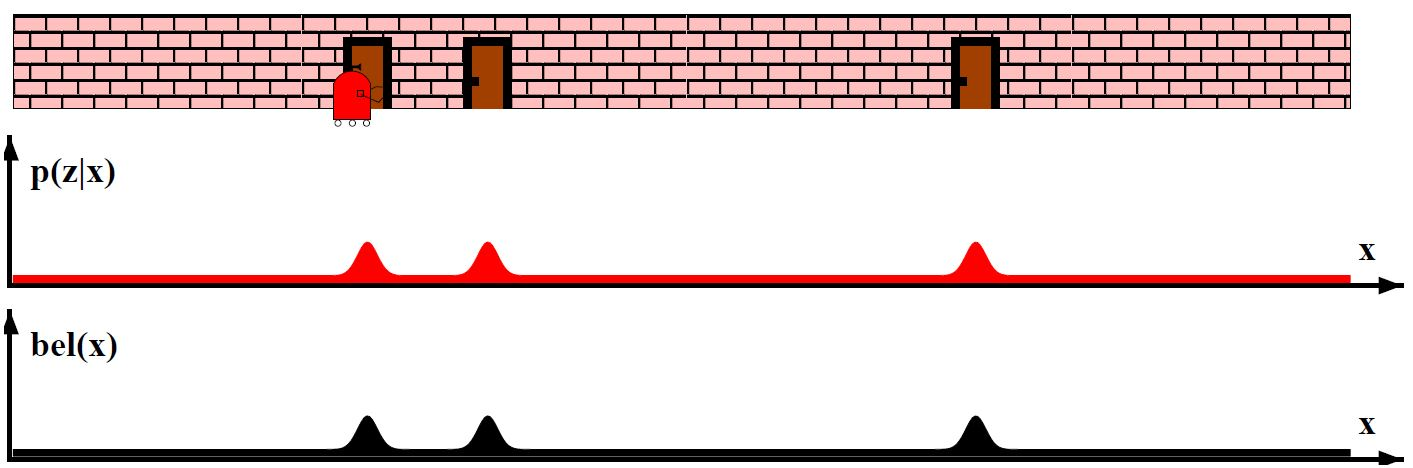
\includegraphics[scale=0.37]{images/MarkovLocalizationB}
\caption{The robot's belief after sensing}
\label{fig:afterSenseBelief}
\end{figure}

\begin{figure}[h]
\centering
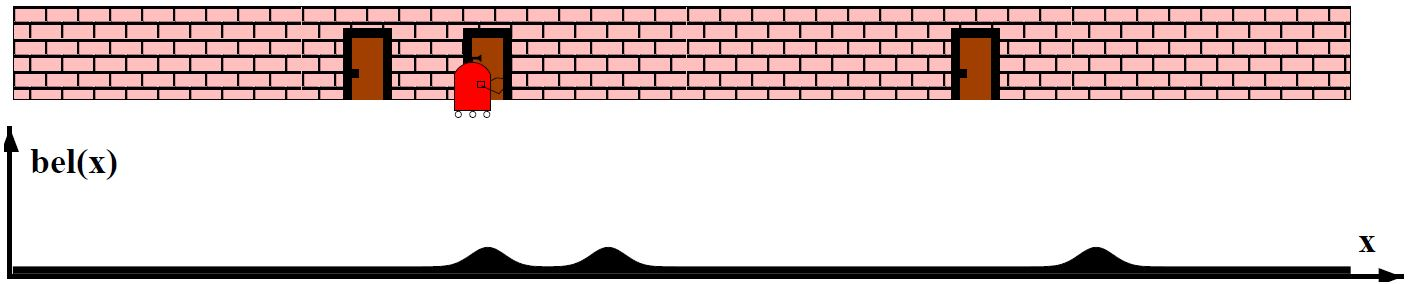
\includegraphics[scale=0.37]{images/MarkovLocalizationC}
\caption{The robot's belief after moving}
\label{fig:afterMoveBelief}
\end{figure}

\begin{figure}[h]
\centering
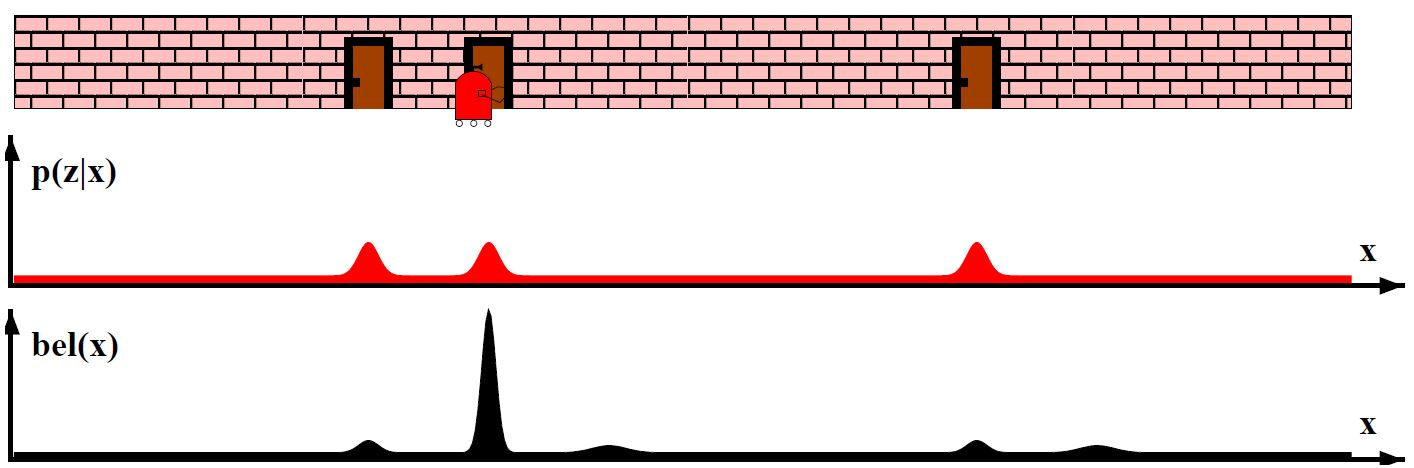
\includegraphics[scale=0.37]{images/MarkovLocalizationD}
\caption{The robot's belief after second sensing}
\label{fig:afterSecondSenseBelief}
\end{figure}

\begin{figure}[h]
\centering
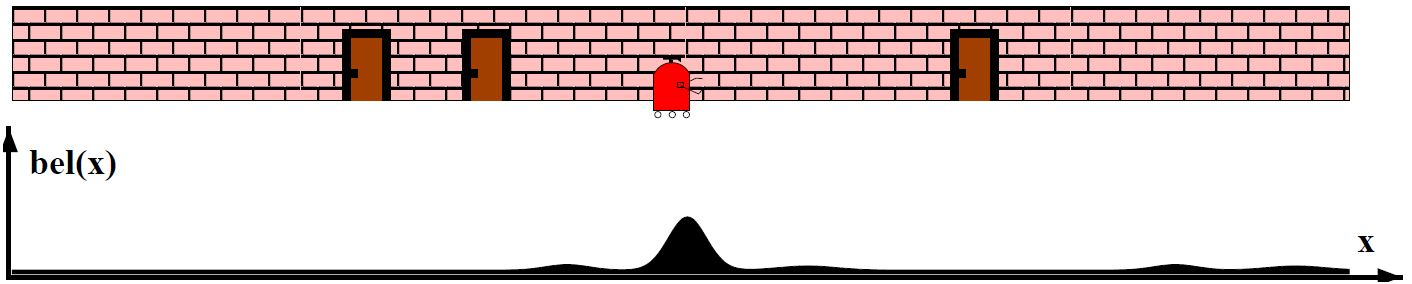
\includegraphics[scale=0.37]{images/MarkovLocalizationE}
\caption{The robot localizes itself}
\label{fig:finalBelief}
\end{figure}